\documentclass[10pt]{article}

% --- Minimal, portable preamble: standard article class, no journal-specific
% class file. No official Aperture Neuro LaTeX/Overleaf template could be
% located at drafting time (their author-guidelines page is JS-rendered and
% not indexable); confirm citation style and any required class file with
% the editor before final submission and adjust \bibliographystyle if needed.

\usepackage[utf8]{inputenc}
\usepackage[T1]{fontenc}
\usepackage{lmodern}
\usepackage[margin=1in]{geometry}
\usepackage{graphicx}
\usepackage{xcolor}
\usepackage{amsmath,amssymb}
\usepackage{booktabs}
\usepackage[colorlinks=true,linkcolor=blue,citecolor=blue,urlcolor=blue]{hyperref}
\usepackage[round]{natbib}
\usepackage{parskip}
\usepackage{orcidlink}

\title{PRISM: a BIDS-compatible metadata and workflow toolkit for psychological experiment datasets}

\author{
  Karl Koschutnig\orcidlink{0000-0001-6234-0498}\\
  \small MRI-Lab Graz, Department of Psychology, University of Graz, Graz, Austria\\
  \small \texttt{karl.koschutnig@uni-graz.at}
}
\date{}

\begin{document}
\maketitle

\begin{abstract}
Psychological and behavioral studies often combine neuroimaging with
questionnaires, participant metadata, physiological recordings, eye tracking,
and other tabular measurements. The Brain Imaging Data Structure (BIDS)
provides an effective baseline for organizing neuroimaging datasets and
associated behavioral files \citep{gorgolewski2016bids}, but many psychology
workflows still depend on ad hoc spreadsheets, incomplete codebooks, and
lab-specific conventions for instrument metadata, response levels, and
derived scores. PRISM is a local-first, open-source toolkit for converting,
validating, and documenting psychological experiment datasets while
remaining compatible with BIDS. It extends BIDS with additional
schema-driven metadata for surveys, biometrics, physiological recordings,
eye tracking, and environment/context files, additively rather than
replacing core BIDS conventions. We describe PRISM's design, and present
validation evidence from a seeded, synthetic adversarial test suite that
exercises the conversion and validation pipeline against 59 deliberately
hostile inputs.
\end{abstract}

\section{Introduction}

Reproducible psychology requires more than stable filenames. Researchers
need machine-readable descriptions of survey items, response options,
reverse coding, units, acquisition settings, participant variables, and
instrument versions. In practice, these details are often scattered across
spreadsheets, survey platform exports, protocol documents, and manuscript
drafts. This creates ambiguity during reanalysis, cross-study comparison,
and long-term reuse.

The gap becomes especially visible in mixed-modality studies. A
BIDS-formatted imaging dataset may be structurally correct while still
lacking the metadata needed to interpret repeated questionnaire
administrations, compare two versions of the same instrument, harmonize
participant variables, or regenerate derived scores. These problems are not
only about validation; they are also about conversion, template reuse, and
keeping metadata synchronized with the data that produced it.

PRISM addresses this need by providing a single workflow layer for
psychology-oriented metadata on top of BIDS. It offers schema-based
validation for additional modalities, converters from common tabular and
survey exports, reusable instrument templates, recipe-based scoring,
participants.tsv generation, and manuscript-facing outputs such as methods
boilerplate. The intended users are researchers, data stewards, and tool
developers who want richer guarantees for behavioral metadata without
giving up compatibility with established BIDS tooling.

\section{State of the field}

PRISM complements rather than replaces established tools in the BIDS
ecosystem. The official BIDS Validator and the broader BIDS standard are
essential for core structural compliance, especially for imaging data
\citep{gorgolewski2016bids}. BIDS \texttt{phenotype/} tables offer a useful
flat representation of participant-level measurements, but they cannot
retain all session, run, and acquisition-variant context for repeated
instrument administrations. PRISM therefore uses subject-, session-, and
run-resolved survey files as its native representation, while providing an
optional, deliberately lossy \texttt{phenotype/} bridge for compatibility
with existing BIDS workflows. PRISM adds checks for item-level metadata,
recipe-based scoring rules, and project-facing conversion workflows that the
BIDS Validator does not attempt to enforce. DataLad is highly effective for
dataset versioning, provenance, distribution, and nested dataset management
\citep{halchenko2021datalad}, but it is not designed to define domain
schemas for psychological instruments or to normalize questionnaire exports
into BIDS-compatible tabular layouts.

Survey collection platforms such as LimeSurvey solve a different problem
again: they help author and administer instruments, but they do not by
themselves produce a reusable research dataset with BIDS-style naming,
sidecars, schema validation, participants harmonization, and derivative
generation. PRISM was therefore developed as a separate toolkit because the
scholarly contribution lies in integrating these concerns: additive BIDS
compatibility, psychology-oriented schemas, template libraries, conversion,
scoring, and export in one reproducible workflow. Contributing isolated
pieces of this functionality upstream would not by itself provide the
end-to-end workflow needed by the target users.

\section{Software design}

PRISM follows four design principles.

\textbf{Additive BIDS compatibility.} PRISM-specific files live alongside
standard BIDS content, and \texttt{.bidsignore} support allows standard BIDS
tools to ignore PRISM-only artifacts when necessary. This makes it possible
to retain acquisition context in native survey files while keeping BIDS apps
usable.

\textbf{Metadata as an executable contract.} Survey and biometrics templates
separate instrument identity and item definitions from study-specific
administration details. Versioned JSON schemas, a registry of instrument
identifiers and citations, and declarative entity rules provide one
machine-readable basis for conversion, filename construction, and
validation. This supports multilingual templates, instrument variants, and
version-aware scoring without requiring researchers to reconstruct those
decisions from spreadsheet conventions. Most bundled survey templates are
derived from the PsyToolkit survey library
\citep{stoet2010psytoolkit,stoet2017psytoolkit}; each template's metadata
records the upstream licensing statement verbatim, and instruments with
unclear or restrictive terms are excluded rather than shipped (103 survey
and one biometrics template at the time of writing).

\textbf{Interactive assistance separated from portable enforcement.} PRISM
Studio guides authoring and conversion (Figure~\ref{fig:studio}), whereas
core schema, validation, and scoring operations are available through CLI
workflows. The standalone \texttt{prism-validator} runs PRISM checks with
optional BIDS validation, template-library validation, safe fix previews,
and JSON, JUnit, SARIF, Markdown, or CSV reports. It is distributed as a
lightweight Docker image and GitHub Action so that datasets can be checked
before sharing and in continuous integration.

\textbf{Auditable derived data and sharing decisions.} Recipe outputs
include derivative metadata and per-recipe provenance sidecars recording the
recipe identifier and version, PRISM version, timestamp, and SHA-256 hashes
of input files. DataLad support is optional, but records scoped changes when
used. The sharing workflow validates selected content before export and can
randomize participant identifiers, mask copyrighted question text, scrub
sensitive MRI sidecar fields, or apply anatomical defacing to the export
copy. It prepares reusable project templates, analysis-oriented exports, and
repository packages such as Austrian NeuroCloud submissions; optional
openMINDS metadata export supports semantic sharing.

\begin{figure}[htbp]
  \centering
  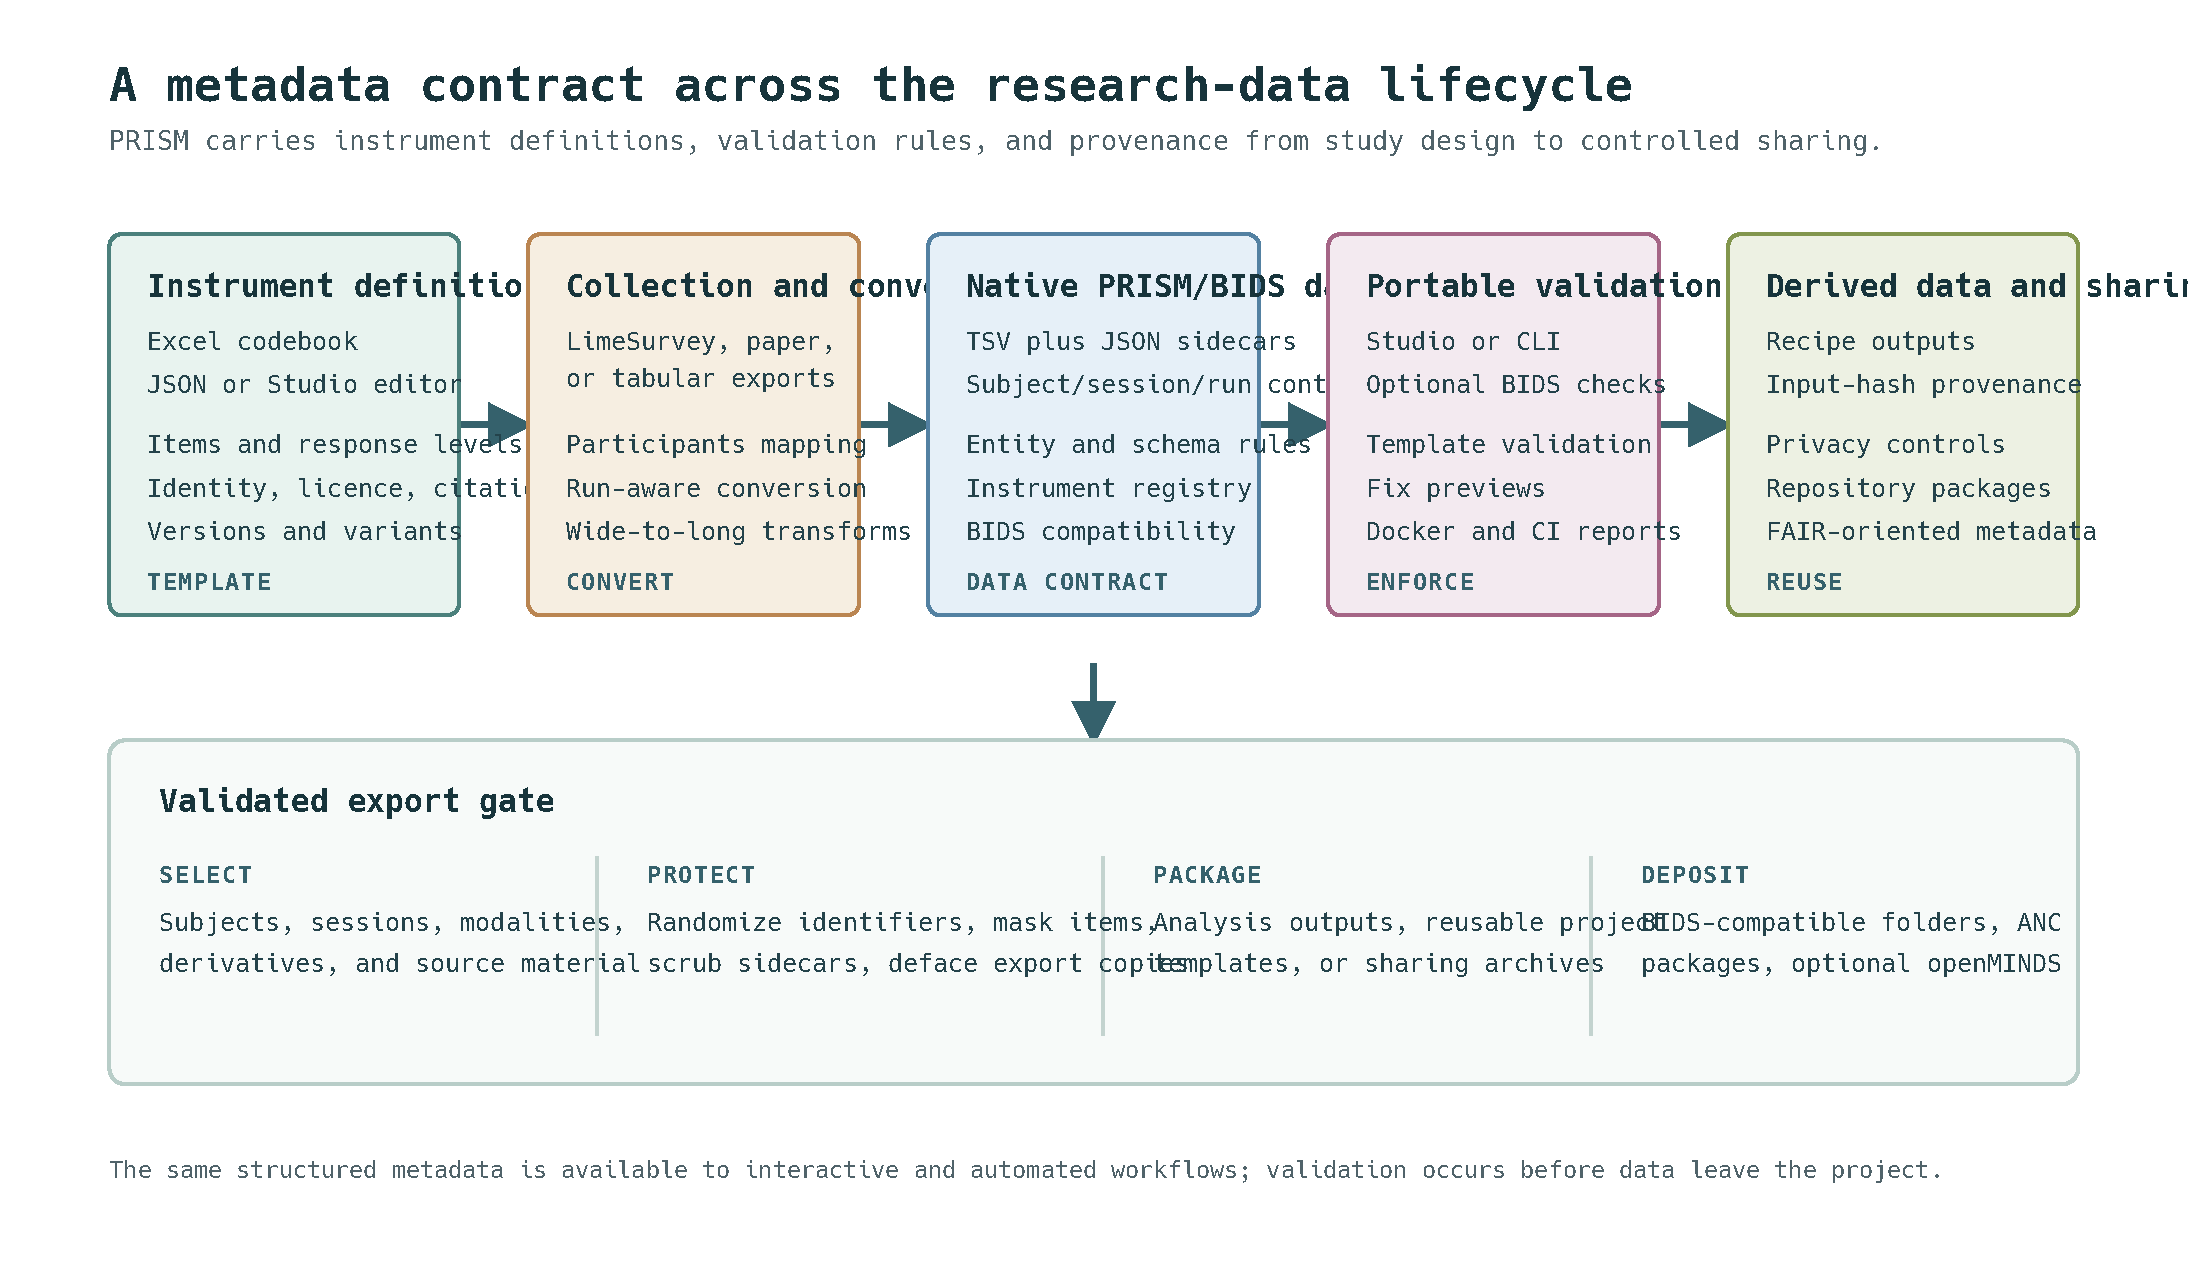
\includegraphics[width=0.85\textwidth]{prism_lifecycle.pdf}
  \caption{PRISM lifecycle: reusable instrument definitions become versioned
  templates, guide data collection and conversion into native PRISM/BIDS
  datasets, are enforced by interactive and automated validation, and
  produce provenance-bearing derivatives and privacy-controlled sharing
  packages.}
  \label{fig:lifecycle}
\end{figure}

\begin{figure}[htbp]
  \centering
  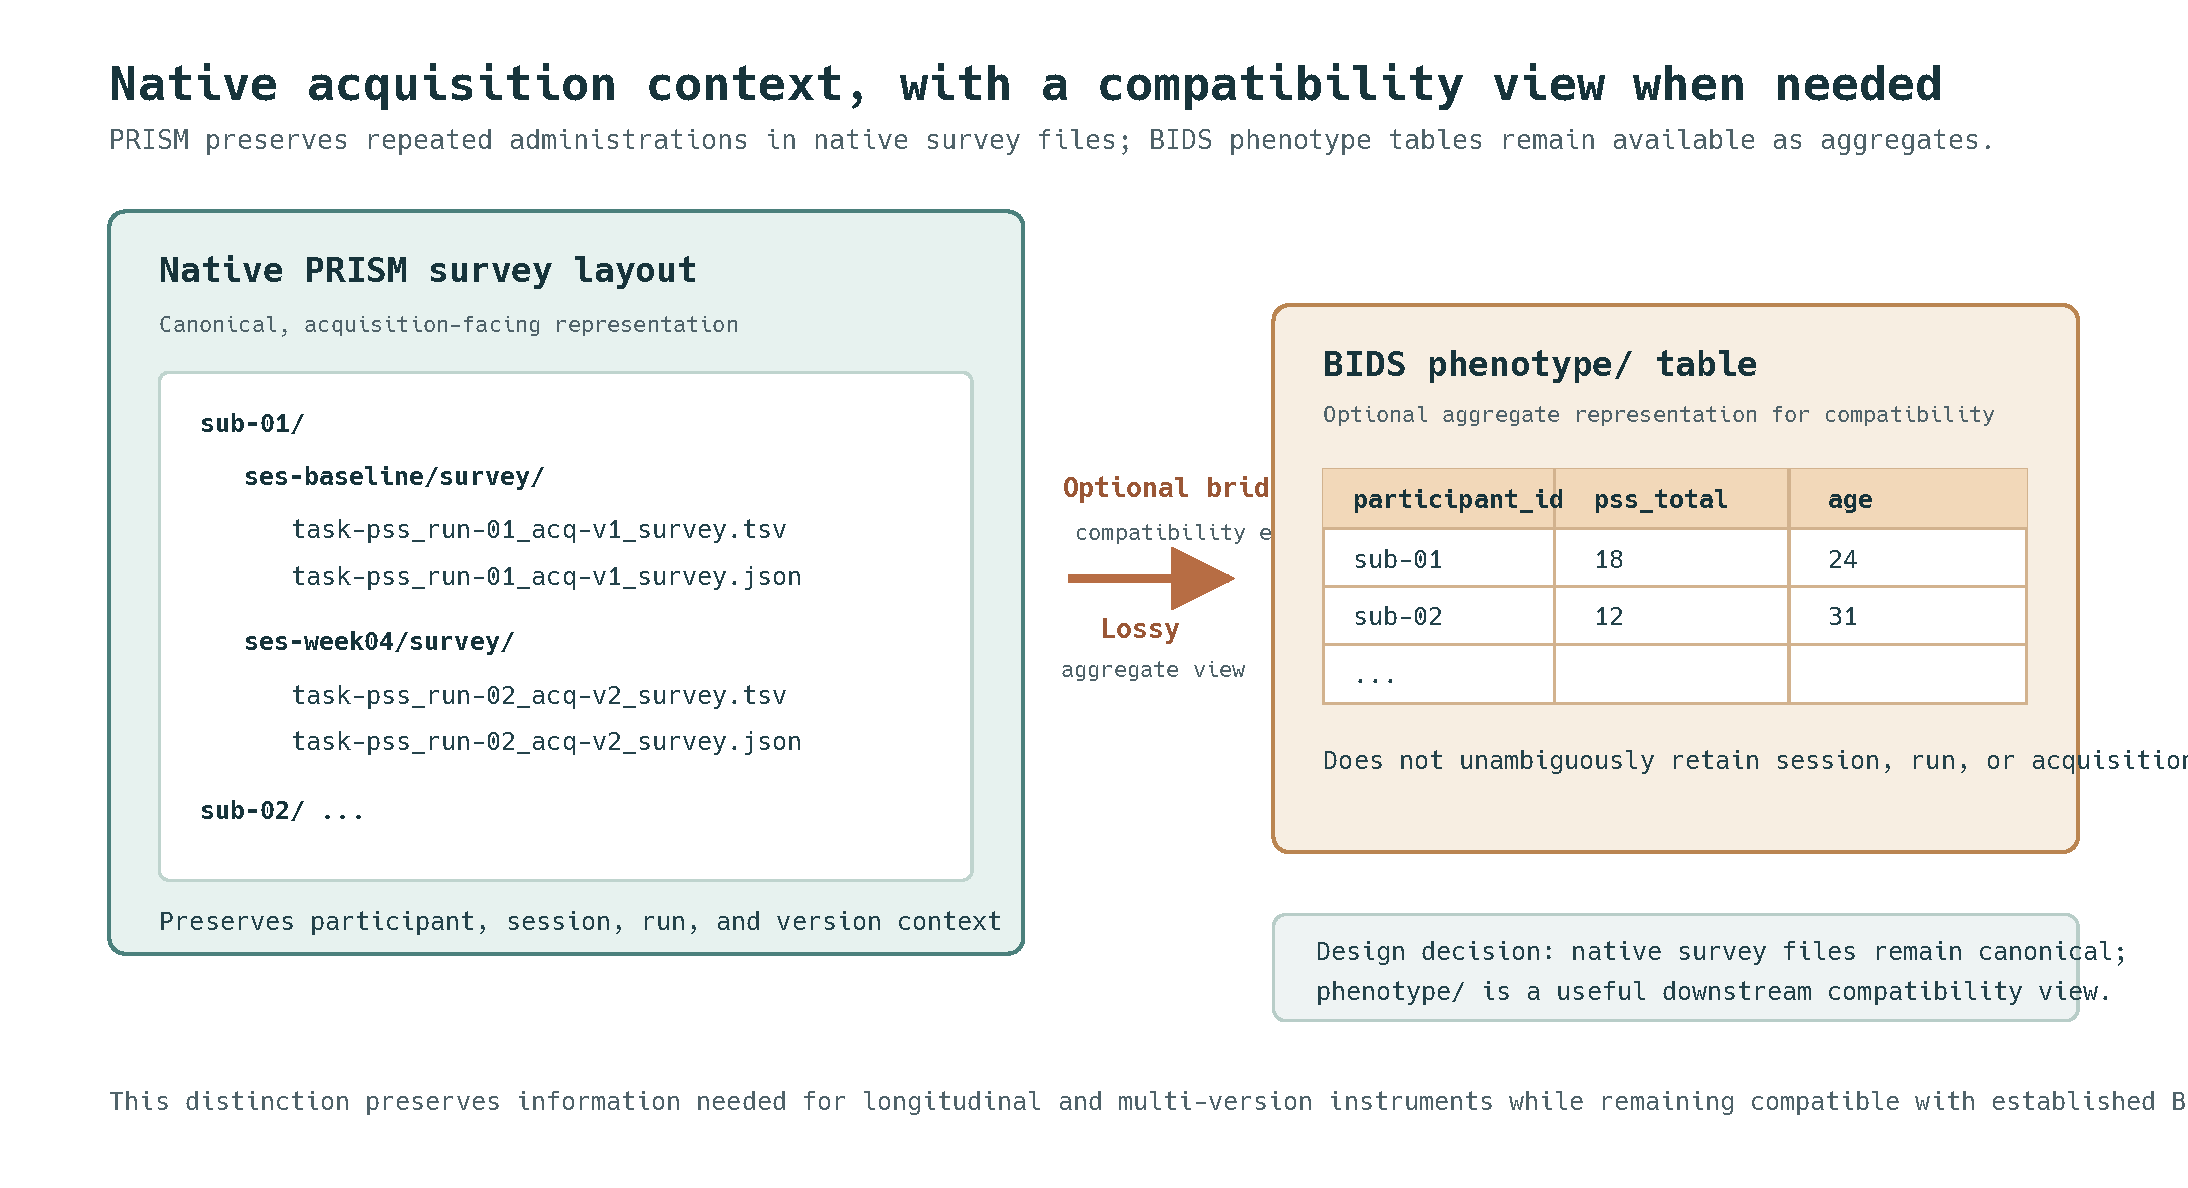
\includegraphics[width=0.85\textwidth]{prism_representations.pdf}
  \caption{PRISM's native survey representation preserves participant,
  session, run, and acquisition-version context. The optional BIDS
  \texttt{phenotype/} bridge creates a compatible aggregate view, but
  intentionally cannot retain all of that acquisition detail.}
  \label{fig:representations}
\end{figure}

\begin{figure}[htbp]
  \centering
  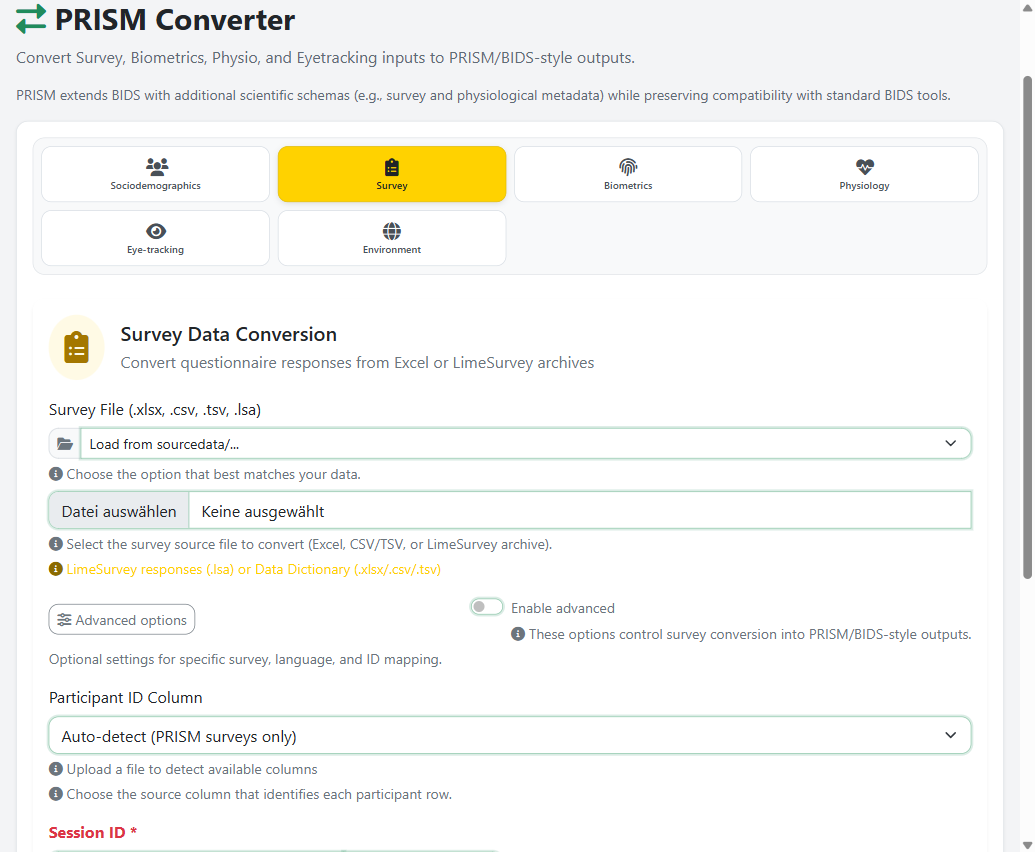
\includegraphics[width=0.8\textwidth]{figure_studio.png}
  \caption{PRISM Studio's survey conversion screen, one of six guided
  converters (sociodemographics, survey, biometrics, physiology,
  eye-tracking, environment) that wrap the same schema-driven conversion and
  validation pipeline exercised in Section~\ref{sec:validation}.}
  \label{fig:studio}
\end{figure}

\section{Validation evidence}
\label{sec:validation}

A recurring weakness in software papers is asserting correctness without
demonstrating it. PRISM's test suite includes a deterministic, seeded
adversarial dataset generator (\texttt{prism\_tools dataset
build-hostile-demo}) that is entirely synthetic: no real participant data is
used or required. Given a fixed random seed, it constructs 59 deliberately
hostile cases across nine pipeline domains --- sociodemographics,
biometrics, environment/MRI sidecar timestamps, subject and session
identifiers, BIDS entity rewriting, recipe/scoring definitions,
input-format diversity (character encodings, spreadsheet formula-like
strings), full survey conversion runs, and participants-table merging.
Each case documents an expected pipeline outcome, for example:

\begin{itemize}
  \item three participants use session labels \texttt{ses-1},
  \texttt{ses-01}, and \texttt{ses-pre} for the same subject, which must
  remain three distinct, uncoerced session labels through every pipeline
  stage rather than being treated as equivalent;
  \item a subject directory named with a non-ASCII character
  (\texttt{sub-M\"uller}) must be handled without the pipeline crashing;
  \item conflicting recipe definitions (an unresolvable formula reference, an
  invalid \texttt{Kind}, a missing required field) must be rejected by
  recipe validation with a clear error rather than silently producing a
  wrong score;
  \item malformed or ambiguous MRI sidecar timestamps (an invalid calendar
  date, a Daylight Saving Time transition, a non-existent leap day) must
  fail to parse cleanly rather than raising an unhandled exception.
\end{itemize}

Thirty-four automated tests assert these documented outcomes case-by-case
and run in continuous integration on every commit, so a regression in any of
the 59 cases is caught immediately rather than discovered by a user.

As an end-to-end illustration for this manuscript, we additionally built the
full synthetic dataset from the same seed and ran both PRISM's own validator
and the official BIDS Validator against the resulting project
(\texttt{prism-validator examples/hostile\_demo --bids}), reproducible with
one command. Table~\ref{tab:validation} reports the result.

\begin{table}[htbp]
  \centering
  \caption{Findings from running PRISM's validator (with BIDS validation
  enabled) against the seeded synthetic adversarial dataset. ``Fixture
  artifact'' rows are a byproduct of the dataset containing MRI JSON
  sidecars without paired imaging binaries (kept out of the repository to
  avoid bundling synthetic binary data), not an injected condition under
  test.}
  \label{tab:validation}
  \begin{tabular}{@{}llrl@{}}
    \toprule
    Code & Layer & Count & Interpretation \\
    \midrule
    \texttt{PRISM601} & PRISM heuristic & 3 & Correctly flagged as
      \emph{potential} session-label typos (\texttt{ses-02}, \texttt{ses-1},
      \texttt{ses-pre}) without merging or coercing the underlying labels. \\
    \texttt{BIDS\_INVALID\_ENTITY\_LABEL} & BIDS spec & 1 & Correctly caught
      the non-ASCII \texttt{sub-M\"uller} label as a genuine BIDS
      specification violation. \\
    \texttt{BIDS\_SIDECAR\_WITHOUT\_DATAFILE} & BIDS spec & 23 & Fixture
      artifact (see caption). \\
    \texttt{BIDS\_NOT\_INCLUDED} & BIDS spec & 1 & Fixture artifact: the
      generated demo guide file at the dataset root. \\
    \bottomrule
  \end{tabular}
\end{table}

The result demonstrates the intended two-layer behavior: PRISM's
domain-specific heuristics surface plausible metadata problems without
silently altering the data they describe, while the official BIDS Validator
independently catches a real specification violation injected by the same
synthetic dataset. This is offered as reproducible, code-verified evidence
of correct behavior on adversarial input, not as evidence of independent
third-party adoption; see Section~\ref{sec:impact} for the latter.

\section{FAIR-oriented dataset preparation}

PRISM supports FAIR-oriented dataset preparation \citep{wilkinson2016fair},
but does not make a dataset FAIR automatically. Findability is supported by
BIDS-style names, versioned schemas, instrument identifiers, keywords, and
DOI/citation fields. Standard JSON, TSV, and CSV formats, BIDS alignment,
optional \texttt{phenotype/} and openMINDS exports, licensing metadata, and
recipe provenance support accessibility, interoperability, and reuse. Actual
access conditions, consent, licensing, and repository deposition remain the
responsibility of the dataset owners.

\section{Research impact statement}
\label{sec:impact}

PRISM has supported a research-data workflow for the Austrian NeuroCloud
dataset \emph{Creativity: a (white) matter of connectivity}
\citep{koschutnig2026creativity}. Its public metadata record identifies
PRISM Studio version 1.15.2 as the creation tool; the authors used PRISM to
enrich the mixed-modality BIDS dataset with metadata and validate it before
repository submission. This is documented author/developer use rather than
evidence of independent adoption, and the dataset remains access-restricted
under the Austrian NeuroCloud data-use agreement.

The public repository shows iterative development from September 2025
onward, tagged releases through version 1.18.0, automated continuous
integration, and cross-platform release artifacts for macOS, Windows, and
Linux. The repository also includes workshop materials, example datasets
(including the synthetic adversarial dataset described in
Section~\ref{sec:validation}), and end-to-end documentation so that
researchers can test the workflows locally rather than treating the software
as an opaque web service.

The scientific value of PRISM is its attempt to make structured behavioral
metadata operational in day-to-day research practice. The bundled template
library, participants and NeuroBagel workflows, survey version handling,
wide-to-long reshaping, LimeSurvey integration, and repository-facing
exports reduce the amount of manual metadata reconciliation required to move
from raw collection outputs to reusable datasets. This is particularly
relevant for labs that already use BIDS for imaging data but still manage
questionnaires and participant metadata in less standardized ways.

\section{Availability and reproducibility}

PRISM is released under the GNU Affero General Public License v3.0
(AGPL-3.0) and developed at
\url{https://github.com/MRI-Lab-Graz/prism-studio}. The release described
here is version 1.18.0. Source installation is documented for macOS,
Windows, and Linux through \texttt{setup.sh} and \texttt{setup.ps1}; entry
points include \texttt{python prism-studio.py} for the web application and
\texttt{prism-validator} for portable validation. The validator is also
distributed as platform bundles, a Docker image, and a GitHub Action. The
repository contains example datasets and workshop material under
\texttt{examples/}, while automated checks are run in CI through
\texttt{python tests/verify\_repo.py} and pytest-based verification. The
bundled instrument library is third-party content rather than PRISM's own
code and is licensed separately; see the library's own notice for
provenance and per-instrument terms.

This manuscript should cite the archival DOI for the exact release under
review once the corresponding Zenodo snapshot has been created.

\section{Data availability statement}

No new participant data are reported in this manuscript. All software,
example datasets, and the synthetic adversarial dataset used in
Section~\ref{sec:validation} are openly available at
\url{https://github.com/MRI-Lab-Graz/prism-studio} under AGPL-3.0 (software)
and the instrument library's own license (templates); an archival DOI will
be added upon acceptance. The Austrian NeuroCloud dataset referenced in
Section~\ref{sec:impact} is access-restricted under its data-use agreement
and is cited, not deposited, here.

\section{Declaration of interest}

The author declares no competing interests.

\section{AI usage disclosure}

Claude Sonnet 5 and GitHub Copilot were used to assist with code drafting
and refactoring, documentation editing, and manuscript drafting and editing.
The GitHub Copilot model and version were not recorded. The author reviewed
all AI-assisted outputs, accepts full responsibility for the manuscript and
software, and retained control of the substantive software-design and
scientific framing decisions.

\section*{Acknowledgements}

The author thanks the MRI-Lab Graz community for testing, issue reports,
and feedback during PRISM's development. We are grateful to the BIDS
community for the standards ecosystem on which PRISM builds, and to
contributors who provided templates, bug reports, and workflow feedback.
This work was conducted at the University of Graz, Austria.

\bibliographystyle{apalike}
\bibliography{paper}

\end{document}
